
\begin{frame}[noframenumbering]{Mouvement de marche}
    \begin{columns}
        \begin{column}{0.4\textwidth}
            \begin{itemize}
                \item Générateur \textit{IKWalk} boucle ouverte + stabilisation
                \item Holonome
                \item Réglage manuel par expérimentation
                \item Mouvement désiré $\neq$ mesuré
                \item Amélioration 2017 : générateur \textit{QuinticWalk}
            \end{itemize}
        \end{column}
        \begin{column}{0.6\textwidth}
            \centering
            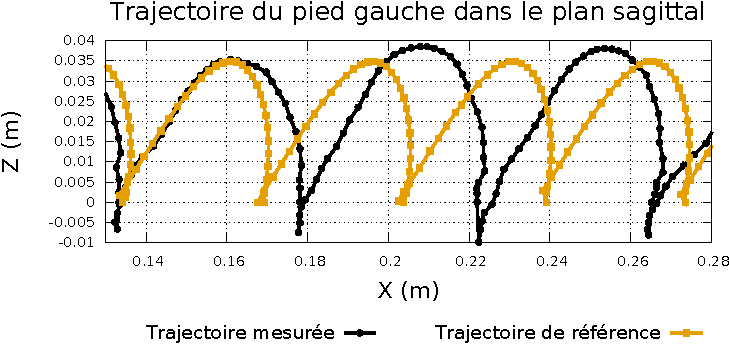
\includegraphics[type=pdf,ext=.pdf,read=.pdf,width=1.0\linewidth]{../plot/walk_traj_foot}
        \end{column}
    \end{columns}
    \vspace{0.2cm}
    \begin{block}{}
        \customtextcolor{
            \small
            \textit{Rhoban hardware and software open source contributions for robocup humanoids}}\\
        \scriptsize
        Quentin Rouxel, Grégoire Passault, Ludovic Hofer, Steve N'Guyen, Olivier Ly\\
        Workshop on Humanoid Soccer Robots, 2015\\
    \end{block}
\end{frame}

\begin{frame}[noframenumbering]{Mouvement de marche (2/3) -- Générateur \textit{IKWalk}}
    \centering
    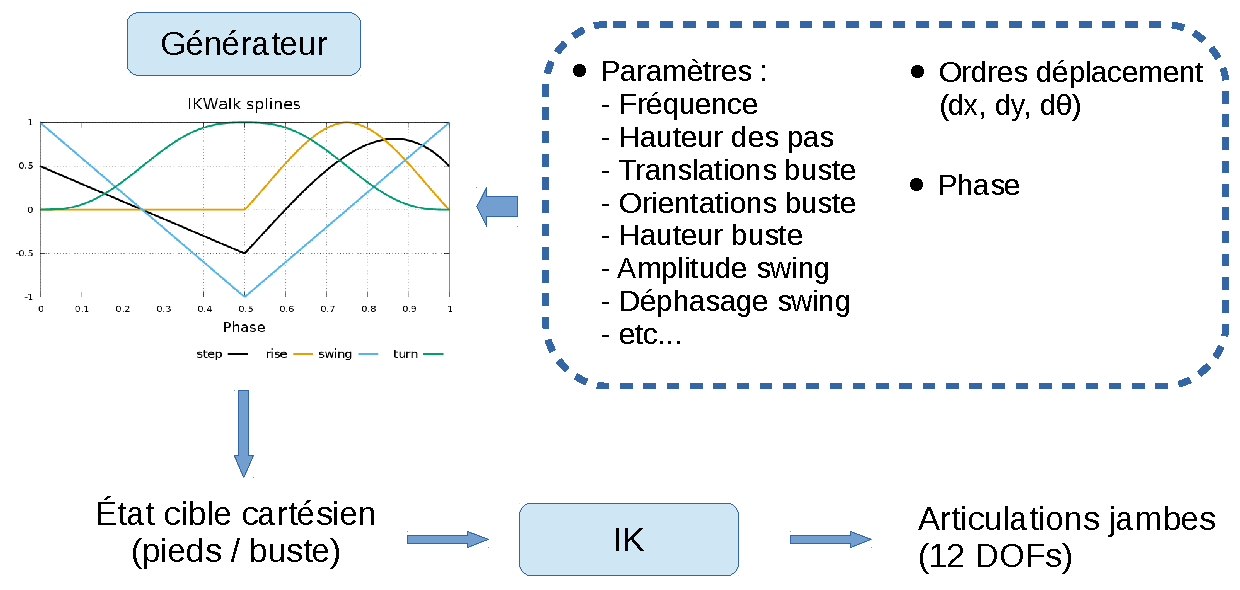
\includegraphics[type=pdf,ext=.pdf,read=.pdf,width=1.0\linewidth]{../schema/ikwalk}
    \begin{block}{}
        \customtextcolor{
            \small
            \textit{Rhoban hardware and software open source contributions for robocup humanoids}}\\
        \scriptsize
        Quentin Rouxel, Grégoire Passault, Ludovic Hofer, Steve N'Guyen, Olivier Ly\\
        Workshop on Humanoid Soccer Robots, 2015\\
    \end{block}
\end{frame}

\begin{frame}[noframenumbering]{Mouvement de marche (3/3) -- Stabilisation}
    \begin{columns}
        \begin{column}{0.5\textwidth}
            \begin{itemize}
                \item Stabilisation latérale
                \item Position du centre de pression
                \item Mise en pause du mouvement
            \end{itemize}
        \end{column}
        \begin{column}{0.5\textwidth}
            \centering
            \movie[
                autostart,
                width=\linewidth, 
                height=0.56\linewidth,
                poster,
                loop
            ]{}{../video/cutStabilization_light.mp4}
            \scriptsize
            (Source : Grégoire Passault)
        \end{column}
    \end{columns}
    \centering
    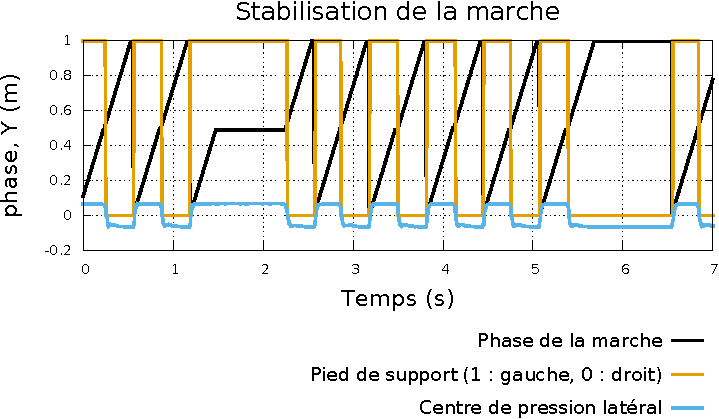
\includegraphics[type=pdf,ext=.pdf,read=.pdf,width=0.6\linewidth]{../plot/walk_stabilization1}
\end{frame}
